%---------change this for every latex homework
\def\yourid{mst3k}
\def\collabs{list collaborators's computing IDs}
\def\sources{Cormen, et al, Introduction to Algorithms.  \emph{(add others here)}}
% -----------------------------------------------------
\def\duedate{Tuesday, May 3, 2022 at {\bf 11:30 pm}}
\def\duelocation{via Gradescope}
\def\htype{Basic}
\def\hunit{D}
\def\hnumber{1}
\def\course{{cs4102 - algorithms - spring 2022}}%------
%-------------------------------------
%-------------------------------------

\documentclass[10pt]{article}
\usepackage[colorlinks,urlcolor=blue]{hyperref}
\usepackage[osf]{mathpazo}
\usepackage{amsmath,amsfonts,graphicx}
\usepackage{latexsym}
\usepackage[top=1in,bottom=1.4in,left=1.25in,right=1.25in,centering,letterpaper]{geometry}
\usepackage{color}
\definecolor{mdb}{rgb}{0.1,0.6,0.4} 
\definecolor{cit}{rgb}{0.05,0.2,0.45} 
\pagestyle{myheadings}
\markboth{\yourid}{\yourid}
\usepackage{clrscode}
\usepackage{listings}
\usepackage{pbox}
\usepackage{tikz}
\usepackage{enumitem}

\newenvironment{proof}{\par\noindent{\it Proof.}\hspace*{1em}}{$\Box$\bigskip}
\newcommand{\handout}{
   \renewcommand{\thepage}{Unit \hunit: \htype~Homework \hnumber~-~\arabic{page}}
   \noindent
   \begin{center}
      \vbox{
    \hbox to \columnwidth {\sc{\course} \hfill}
    \vspace{-2mm}
       \hbox to \columnwidth {\sc due \MakeLowercase{\duedate} \duelocation\hfill {\Huge\color{mdb}\hunit\hnumber{\Large\MakeLowercase{\htype}}(\yourid)}}
      }
   \end{center}
   \vspace*{1mm}
   \hrule
   \vspace*{1mm}
    {\footnotesize \textbf{Collaboration Policy:} You are encouraged to collaborate with up to 3 other students, but all work submitted must be your own {\em independently} written solution. List the computing ids of all of your collaborators in the \texttt{collabs} command at the top of the tex file. Do not share written notes, documents (including Google docs, Overleaf docs, discussion notes, PDFs), or code.  Do not seek published or online solutions for any assignments. If you use any published or online resources (which may not include solutions) when completing this assignment, be sure to cite by naming the book etc.\ or listing a website's URL. Do not submit a solution that you are unable to explain orally to a member of the course staff. Any solutions that share similar text/code will be considered in breach of this policy. Please refer to the syllabus for a complete description of the collaboration policy.
   \vspace*{1mm}
    \hrule
    \vspace*{2mm}
    \noindent
    \textbf{Collaborators}: \collabs\\
    \textbf{Sources}: \sources}
    \vspace*{2mm}
    \hrule
    \vskip 2em
}

\newcommand{\solution}[1]{\color{blue}\hfill\break\noindent\textbf{Solution:} #1\color{black}}
\newcommand{\altsolution}[1]{\color{blue}\hfill\break\noindent\textbf{Solution (Alternative):} #1\color{black}}

%\newcommand{\solution}[1]{}
%\newcommand{\altsolution}[1]{}

\newcommand{\bit}[1]{\{0,1\}^{ #1 }}
%\dontprintsemicolon
%\linesnumbered
\newtheorem{problem}{\sc\color{cit}problem}
\newtheorem{practice}{\sc\color{cit}practice}
\newtheorem{lemma}{Lemma}
\newtheorem{definition}{Definition}
\newtheorem{theorem}{Theorem}

\newcommand{\Z}{\mathbb{Z}} % This might be useful for Integers!

\begin{document}
\thispagestyle{empty}
\handout

%----Begin your modifications here.  Add your answer in the \solution environment for each question


\begin{problem} True or False. (You don't have to explain this in your submission, but you should understand the reason behind your answer.)  \end{problem}

\begin{enumerate}
\renewcommand{\theenumi}{\Alph{enumi}}

\item When the \emph{Ford-Fulkerson} algorithm completes, each back-flow edge from $v$ back to $u$ in the residual graph $G_f$ represent the final flow values for edge $(u,v)$ in the flow-graph $G$.
\solution{
    Your answer here!
}

\item In a standard network flow-graph, under certain conditions a vertex $v$ that is not the source or the sink can have total in-flow that has a different value than its total out-flow.
\solution{
    Your answer here!
}

\item In \emph{Ford-Fulkerson}, for a pair of vertices $u$ and $v$ connected in the residual capacity graph $G_f$, the sum of the values for the back-flow and the residual capacity edges between that vertex-pair must always equal the capacity of the edge between them in the flow-graph $G$.
\solution{
    Your answer here!
}

\item When using Ford-Fulkerson, if there is no augmenting path in $G_f$, then there exists a cut in $G$ whose capacity equals $f$, the max-flow value for graph $G$.
\solution{
    Your answer here!
}


\end{enumerate}



\begin{problem}Max Flow\end{problem}
Given the following Flow Network $G$:

\vskip 2em
\begin{center}
\resizebox{.48\textwidth}{!}{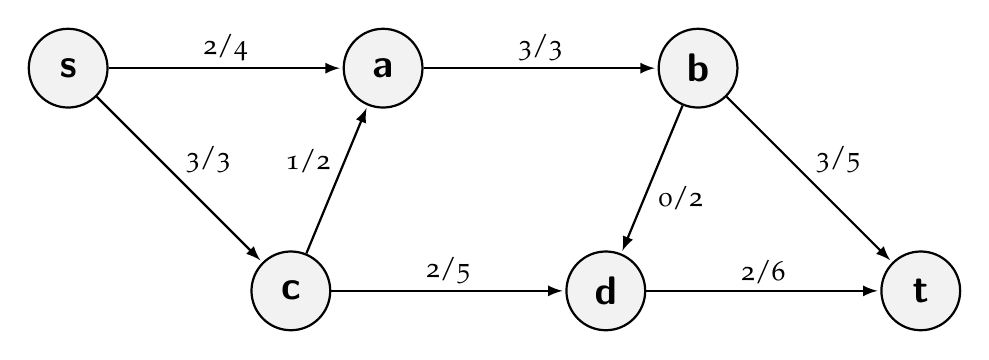
\begin{tikzpicture}[->,>=latex,shorten >=1pt,auto,node distance=4cm,
  thick,main node/.style={circle,fill=gray!10,draw,
  font=\sffamily\Large\bfseries,minimum size=10mm}]
%   \tikzset{edge/.style = {->,> = latex'}}

  \node[main node] (s) {s};
  \node[main node] (a) [right of=s] {a};
  \node[main node] (c) [below right of=s] {c};
  \node[main node] (b) [right of=a] {b};
  \node[main node] (d) [right of=c] {d};
  \node[main node] (t) [below right of=b] {t};

  \path[every node/.style={
        fill=white,inner sep=2pt}]
    % Right-hand-side arrows rendered from top to bottom to
    % achieve proper rendering of labels over arrows.
    (s) edge [] node[] {2/4} (a)
        edge [] node[] {3/3} (c)
    (a) edge [] node[] {3/3} (b)
    (b) edge [] node[] {0/2} (d)
        edge [] node[] {3/5} (t)
    (c) edge [] node[] {1/2} (a)
        edge [] node[] {2/5} (d)
    (d) edge [] node[] {2/6} (t);
\end{tikzpicture}}
\end{center}
\vskip 2em

\begin{enumerate}
    \item Find the Residual Graph $G_f$ for $G$ by listing all the edges in $G_f$ and the numeric value associated with each edge.
    \solution{
    Your answer here!
    }

    \item Find an augmenting path in the graph $G_f$.  List the nodes in the path you found in order (e.g., $s \rightarrow a \rightarrow b \rightarrow t$).
    \solution{
    Your answer here!
    }
    
    
    \item Find the min cut of the graph.  List the nodes below on each side of the cut.
\begin{center}
\begin{tabular}{|c|c|}
     \hline
    \textbf{$S$ (one side)} & \textbf{$V-S$ (other side)}\\
     \hline \hline
     \hspace{2.5in} & \hspace{2.5in} \\
      & \\
      & \\
      & \\
      & \\
      & \\
     \hline
\end{tabular}
\end{center}

\item What is the maximum flow of this graph?
\end{enumerate}

\solution{
Your answer here!
}
  
 
\begin{problem}\end{problem}
We used \emph{Ford-Fulkerson} to solve the \emph{Vertex-Disjoint Paths} problem in class by reducing
\emph{Vertex-Disjoint Paths} to \emph{Edge-Disjoint Paths} and 
\emph{Edge-Disjoint Paths} to \emph{Max Flow}. Recall that a set of vertex-disjoint paths is
a set of edge-disjoint paths where each node is used at most once. How would we modify the reduction from \emph{Vertex-Disjoint Paths} to \emph{Max Flow} if we want to compute a set of edge-disjoint paths where each vertex is used at most {\em twice}? Briefly describe our original reduction and the change(s) you would make. {\bf Note:} If you prefer, you may just modify the reduction from \emph{Vertex-Disjoint Paths} to \emph{Edge-Disjoint Paths}.
\solution{
    Your answer here!
}


\begin{problem}NP Completeness\end{problem}
\begin{enumerate}
    \item We know that $C$ is $NP$-Hard and that $A \in NP$.  Which of these show that $A$ is $NP$-Complete?
    \begin{itemize}
        \item[a)] $A$ reduces to $B$ and $B$ reduces to $C$
        \item[b)] $C$ reduces to $B$ and $B$ reduces to $A$
    \end{itemize}
    \solution{
    Your answer here!
    }

    
    \item Which shows that $P = NP$, given that $A$ reduces to $B$ and $B$ reduces to $C$?
    \begin{itemize}
        \item[a)] $A \in P$ and $C \in NP$-Hard
        \item[b)] $A \in NP$-Hard and $C \in P$
    \end{itemize}
    \solution{
    Your answer here!
    }

\end{enumerate}


\begin{problem} True or False. (You don't have to explain this in your submission, but you should understand the reason behind your answer.)  \end{problem}

\begin{enumerate}
\renewcommand{\theenumi}{\Alph{enumi}}

\item In our reduction of an instance $G$ of the \emph{vertex-disjoint path} problem to an instance $G'$ for \emph{edge-disjoint path} problem, if two paths in $G'$ share a vertex, then the two paths that correspond to those in $G$ must share an edge.
\solution{
Your answer here!
}

\item In our example illustrating bipartite matching, we can tell if every hard-working TA was matched with exactly one adorable dog and \textit{vice versa} by transforming the bipartite graph to a network flow problem and checking if the max-flow $|f| = V$, the total number of vertices in bipartite graph.
\solution{
Your answer here!
}

\item If we find a polynomial solution to a problem in NP, then this proves that $P=NP$.
\solution{
Your answer here!
}

\item If someone proves that a given problem X in NP has an exponential lower bound, then no problem in NP-complete can be solved in polynomial time. 
\solution{
Your answer here!
}

\item It is not possible that an algorithm that solves the 3-CNF problem in polynomial time exists.
\solution{
Your answer here!
}

\end{enumerate}


\begin{problem}Create a Reduction\end{problem}
Reduce \textit{Element Uniqueness} to \textit{Closest Pair of Points} in $O(n)$ time.  Element Uniqueness is defined as: given a list of numbers, return true if no number appears more than once (i.e., every number is distinct).  Closest Pair of Points is defined as: given a list of points $(x,y)$, return the smallest distance between any two points.
\solution{
Your answer here!
}

\begin{problem} Gradescope Submission \end{problem}
Submit a version of this \verb|.tex| file to Gradescope with your solutions added, along with the compiled PDF.  You should only submit your \verb|.pdf| and \verb|.tex| files.

\end{document}

